\section{An explicit surface and its polarization}
\label{sec:surface}

We construct a family of smooth projective surfaces from which we will
choose one violating the inequality established above.  The construction uses the six lines joining
four points of the plane, followed by a cover obtained by taking roots of
their ratios.  The same line arrangement provides the sections needed for
an ample globally generated divisor on the cover.  This choice of
arrangement and polarization is the complete-quadrangle construction
in \cite[Section 7.2]{Anghel2026}; all properties needed here are verified below.

\begin{proposition}\label{prop:surface}
For each prime $n\geq3$, there is a smooth integral projective complex
surface $X$ with an ample globally generated divisor $H$ such that
\[
 H^2=5n^3,\qquad K_X^2-2c_2(X)=n^3(n^2-10).
\]
\end{proposition}

We prove the proposition by constructing the cover, checking its local
coordinates, and then finding sections of the required polarization.
The covering construction goes back to Hirzebruch's work on line
arrangements \cite{Hirzebruch1983}.

\subsection{The branch divisor}

Choose four points $p_1,\ldots,p_4\in\mathbb P^2_{\mathbb C}$, no three
collinear, and let $B$ be their blowup.  Write $\ell$ for the pullback of
the line class and $e_1,\ldots,e_4$ for the exceptional curves.  Thus
\[
 \ell^2=1,\qquad \ell\cdot e_i=0,\qquad
 e_i\cdot e_j=-\delta_{ij},\qquad
 K_B=-3\ell+\sum_{i=1}^4 e_i.
\]
Number the six joining lines from $1$ to $6$, and choose defining linear
forms $l_1,\ldots,l_6$.  Denote the strict transform of line $a$ by $L_a$
and its total transform by $T_a$.  If its endpoints are $p_i,p_j$, then
\[
 T_a=L_a+e_i+e_j\sim\ell.
\]
Two joining lines are called \emph{opposite} if their endpoint pairs are
disjoint.  There are three opposite pairs.

Let
\[
 \Delta=\sum_{a=1}^6 L_a+\sum_{i=1}^4e_i.
\]
This reduced divisor has simple normal crossings.  Each exceptional curve
meets the three incident strict transforms in three distinct points.
Strict transforms of lines with a common endpoint are disjoint, whereas
each opposite pair meets transversely in one point away from the
exceptional curves.  The three latter points are distinct: an equality
between two would force two lines with a common endpoint to meet away
from that endpoint.  Consequently $\Delta$ has ten rational components,
each meeting the others in three points, and fifteen nodes in total.
Figure~\ref{fig:branch-incidence} records these incidences; in the
figure $L_{ij}$ denotes the strict transform of the line joining
$p_i$ and $p_j$.
Since each point belongs to three joining lines,
\begin{equation}\label{eq:branch-class}
 \Delta\sim6\ell-2\sum_{i=1}^4e_i=-2K_B,
 \qquad K_B^2=5.
\end{equation}

\begin{figure}[htbp]
\centering
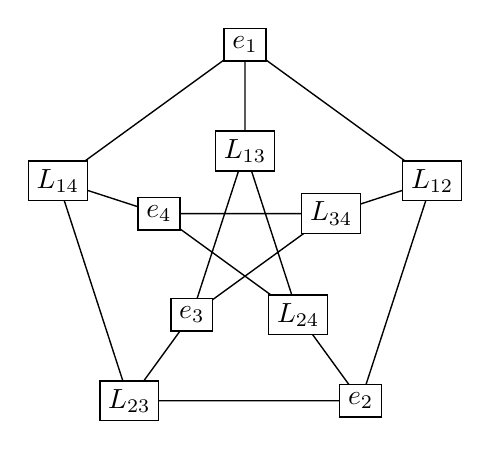
\begin{tikzpicture}[every node/.style={draw,fill=white,inner sep=3pt},
  line width=0.5pt]
\coordinate (outerone) at (90:2.5);
\coordinate (outertwo) at (18:2.5);
\coordinate (outerthree) at (-54:2.5);
\coordinate (outerfour) at (-126:2.5);
\coordinate (outerfive) at (162:2.5);
\coordinate (innerone) at (90:1.15);
\coordinate (innertwo) at (18:1.15);
\coordinate (innerthree) at (-54:1.15);
\coordinate (innerfour) at (-126:1.15);
\coordinate (innerfive) at (162:1.15);
\draw (outerone)--(outertwo)--(outerthree)--(outerfour)--(outerfive)--cycle;
\draw (outerone)--(innerone) (outertwo)--(innertwo)
      (outerthree)--(innerthree) (outerfour)--(innerfour)
      (outerfive)--(innerfive);
\draw (innerone)--(innerthree)--(innerfive)--(innertwo)--(innerfour)--cycle;
\node at (outerone) {$e_1$};
\node at (outertwo) {$L_{12}$};
\node at (outerthree) {$e_2$};
\node at (outerfour) {$L_{23}$};
\node at (outerfive) {$L_{14}$};
\node at (innerone) {$L_{13}$};
\node at (innertwo) {$L_{34}$};
\node at (innerthree) {$L_{24}$};
\node at (innerfour) {$e_3$};
\node at (innerfive) {$e_4$};
\end{tikzpicture}
\caption{The branch-incidence graph on the blown-up plane.
Vertices represent the ten rational components, not points of the
surface; edges represent its fifteen branch nodes. Twelve edges join
$e_i$ to an incident $L_{ij}$, and three join opposite line transforms.
Every vertex has degree three. Crossings of drawn graph edges do not
represent additional intersections.}
\label{fig:branch-incidence}
\end{figure}

\subsection{The cover and its local coordinates}

Fix a prime $n\geq3$, to be chosen at the end.  In an algebraic closure of
$K=\mathbb C(B)$ choose elements $y_a$ satisfying
\[
 y_a^n=l_a/l_6\qquad(1\leq a\leq5),
\]
and let $\pi:X\to B$ be the normalization of $B$ in
$K'=K(y_1,\ldots,y_5)$. The base $B$ is normal and Noetherian, and
this finite characteristic-zero field extension is separable.
Its normalization is therefore finite \cite[Tag~032L]{Stacks},
so $X$ is an integral projective surface.

\begin{lemma}\label{lem:cover-smooth}
The surface $X$ is smooth and $\deg\pi=d=n^5$.  The map is unramified
outside $\Delta$ and has ramification index $n$ along every component of
$\Delta$.  More precisely, near a point at which exactly $s\in\{0,1,2\}$
components of $\Delta$ meet, it is, after an \'{e}tale base change, the
disjoint union of $n^{5-s}$ copies of
\[
 (t_1,t_2)\longmapsto
 \begin{cases}
 (t_1,t_2),&s=0,\\
 (t_1^n,t_2),&s=1,\\
 (t_1^n,t_2^n),&s=2.
 \end{cases}
\]
Here the displayed maps are understood in \'{e}tale coordinates on the
base and the source.
\end{lemma}

\begin{proof}
First, suppose that integers $c_1,\ldots,c_5$ satisfy
\[
 \prod_{a=1}^5(l_a/l_6)^{c_a}\in K^{*n}.
\]
Taking valuations along $L_a$ shows that $n$ divides $c_a$ for every $a$.
Thus the five radicands are independent in $K^*/K^{*n}$.  Since $K$
contains the $n$th roots of unity, the extension $K'/K$ is Galois and its
group embeds in $(\mathbb Z/n)^5$ by its action on the roots.  If its
image were a proper subgroup, some nonzero linear functional on
$(\mathbb Z/n)^5$ would annihilate it.  The corresponding product of
the $y_a$ would then lie in $K$, contradicting the independence just
proved.  This gives $[K':K]=n^5$.

We next record the valuations modulo $n$ along the branch curves.  Use
the vector space
\[
 U_n=\mathbb F_n^6/\langle(1,1,1,1,1,1)\rangle
\]
and denote the images of its six standard vectors by
$\varepsilon_1,\ldots,\varepsilon_6$.  Identifying
$\varepsilon_1,\ldots,\varepsilon_5$ with the standard basis of
$\mathbb F_n^5$, the valuation vector along $L_a$ is
$\varepsilon_a$; in particular
$\varepsilon_6=-\sum_{a=1}^5\varepsilon_a$.  If $I_i$ is the set of
the three lines incident with $p_i$, the valuation vector along $e_i$ is
\[
 w_i=\sum_{a\in I_i}\varepsilon_a.
\]
All these vectors are nonzero.  At a node formed by two strict
transforms, the vectors are two distinct $\varepsilon_a$, hence are
independent.  At a node $L_a\cap e_i$, one has $a\in I_i$, and
$\varepsilon_a,w_i$ are independent as well.  Indeed, if
$\lambda\varepsilon_a+\mu w_i=0$ in $U_n$, a coordinate outside $I_i$
forces the corresponding constant vector to be zero.  A coordinate in
$I_i\setminus\{a\}$ then gives $\mu=0$, followed by $\lambda=0$.

It remains to check that this independence gives the asserted smooth
normalization, including at the nodes.  At a closed point of $B$, choose
regular parameters $u_1,u_2$ such that the local branches of $\Delta$
are $u_1=0,\ldots,u_s=0$.  Shrink to an affine neighborhood on which
these parameters define an \'{e}tale map to $\mathbb A^2$.  Each radicand
is a monomial in $u_1,\ldots,u_s$, with possibly negative exponents,
times a unit.  Adjoining $n$th roots of these units is an \'{e}tale base
change.  On an integral neighborhood of a point of that base change,
divide the $y_a$ by the resulting roots of the units.

The $s$ columns of exponents modulo $n$ are independent by the preceding
calculation.  Multiplicative changes of the five root generators by a
matrix in $\operatorname{GL}_5(\mathbb F_n)$ therefore reduce their
equations to
\[
 Y_j^n=u_j\quad(1\leq j\leq s),\qquad
 Y_j^n=1\quad(s<j\leq5).
\]
To make this reduction in the function field, lift the matrix entries
to integers and divide by suitable monomials in the $u_j$ to remove
exponents divisible by $n$.  The generator change is reversible because
its matrix is invertible modulo $n$.  It consequently describes the
whole generic algebra after base change, not merely a subextension.
The first $s$ equations generate a field of degree $n^s$, by the
valuations along $u_j=0$, and the remaining equations split completely.
The generic algebra is therefore a product of $n^{5-s}$ copies of that
field.

On this neighborhood, with coordinate ring $C$, the normalization in
each factor is
\[
 C[t_1,\ldots,t_s]/(t_1^n-u_1,\ldots,t_s^n-u_s),
\]
so the full normalization is a product of $n^{5-s}$ such algebras.
Indeed, this algebra is finite and free over $C$, has the indicated
generic field, and is smooth: it is the base change of the \'{e}tale
coordinate map to $\mathbb A^2$ along the corresponding coordinate
power map.  In particular it is normal, so it is the integral closure
of $C$ in that field.  Normalization commutes with this \'{e}tale base
change: the pullback of $X$ is normal and has the same generic algebra,
and is pure of dimension two, since it is \'{e}tale over the normal
integral surface $X$. Each component therefore dominates the new
integral base: its finite image is closed and has dimension two.
This proves the local description
and hence the lemma.
\end{proof}

\subsection{The Chern numbers}

The local coordinates in Lemma~\ref{lem:cover-smooth} give both the
canonical divisor formula and the degrees of the coverings of the
branch strata.  Thus no further description of $X$ is needed to compute
its Chern numbers. These calculations recover Hirzebruch's formulas
\cite[Section~2.2, Equations~(5) and (7)]{Hirzebruch1983} for this
six-line arrangement.

The Jacobian of the coordinate power map gives
\[
 K_X\sim_{\mathbb Q}
 \pi^*\bigl(K_B+(1-1/n)\Delta\bigr)
 \sim_{\mathbb Q}(1-2/n)\pi^*(-K_B).
\]
Using \eqref{eq:branch-class} and the degree of $\pi$, we obtain
\begin{equation}\label{eq:cover-canonical}
 K_X^2=5d(1-2/n)^2.
\end{equation}

For the second Chern number, let $e_c$ denote compactly supported
topological Euler characteristic.  The surface $B$ has Euler
characteristic $3+4=7$.  Removing the three nodes from each rational
component of $\Delta$ gives the one-branch stratum $\Delta^\circ$,
whose Euler characteristic is $10(2-3)=-10$.  The node set has fifteen
points.  Additivity therefore gives
\[
 e_c(B\setminus\Delta)=7-(-10)-15=2.
\]
Over the stratum with $s$ branches, the reduced inverse image is a
finite \'{e}tale cover of degree $d/n^s$.  By additivity and
multiplicativity of $e_c$, followed by Chern--Gauss--Bonnet
\cite[Section~1.3 and Proposition~1.6]{Behrend2009},
\begin{equation}\label{eq:cover-euler}
 c_2(X)=e_c(X)
 =d\left(2-\frac{10}{n}+\frac{15}{n^2}\right).
\end{equation}
Subtracting twice \eqref{eq:cover-euler} from
\eqref{eq:cover-canonical} yields
\begin{equation}\label{eq:cover-chern-gap}
 K_X^2-2c_2(X)=d\left(1-\frac{10}{n^2}\right).
\end{equation}

\subsection{An ample globally generated divisor}

To compare \eqref{eq:cover-chern-gap} with the obstruction, we seek an
integral divisor $H$ satisfying $nH\sim\pi^*(-K_B)$.  Such a divisor has
square $5d/n^2$, as required by Proposition~\ref{prop:surface}.  We first
construct $H$ and sections that generate $\mathcal O_X(H)$, and then
prove ampleness separately.  The ramification makes the pullbacks of all
branch components divisible by $n$ as integral divisors.  Put
\[
 R_a=\frac1n\pi^*L_a,\qquad
 F_i=\frac1n\pi^*e_i,\qquad E=\sum_{i=1}^4F_i,
 \qquad J=\frac1n\pi^*T_6.
\]
These are effective Cartier divisors because $X$ is smooth.  If line
$a$ joins $p_i,p_j$, write
\[
 J_a=\frac1n\pi^*T_a=R_a+F_i+F_j.
\]
For $1\leq a\leq5$, the root ratios give
\[
 \operatorname{div}(y_a)=J_a-J.
\]
Since $J_6=J$, all six $J_a$ are linearly equivalent to $J$.  Let $z_a$ be the resulting
sections of $\mathcal O_X(J)$ with zero divisors $J_a$.

These six sections have no common zero.  Away from the exceptional
curves, no point of $B$ lies on all six joining lines.  On an
exceptional curve $e_i$, the total transform of any line not incident
with $p_i$ is disjoint from $e_i$.  Thus the six total transforms have
empty common intersection on $B$, and the same holds for their reduced
pullbacks on $X$.

For an opposite pair $a,b$, its endpoints are the four distinct points,
and hence
\[
 J_a+J_b=R_a+R_b+E.
\]
Dividing $z_az_b$ by the canonical section of $\mathcal O_X(E)$ gives
a section of $\mathcal O_X(2J-E)$ with zero divisor $R_a+R_b$.  These
three sections have no common zero.  In fact the unions $L_a\cup L_b$
belonging to different opposite pairs are disjoint on $B$: a line in
one pair shares an endpoint with every line in either other pair, so
their strict transforms are disjoint.  We have therefore proved that
both $J$ and $2J-E$ are globally generated.  Their sum
\begin{equation}\label{eq:cover-polarization}
 H=3J-E
\end{equation}
is globally generated as well.

To check ampleness, first note that $2\ell-\sum_i e_i$ is globally
generated on $B$ by the three opposite-pair conics: after removing
their exceptional components, their zero divisors are precisely the
three disjoint unions just considered.  Thus this divisor is nef, as
is $\ell$.  The class $\ell$ has positive intersection with every
nonexceptional curve, and
$(2\ell-\sum_i e_i)\cdot e_j=1$ for every exceptional curve.
Consequently
\[
 -K_B=\ell+\left(2\ell-\sum_i e_i\right)
\]
has positive intersection with every integral curve.  Its square is
$5$, so the surface Nakai--Moishezon criterion
\cite[Chapter~V, Theorem~1.10]{Hartshorne} proves that $-K_B$ is
ample. Since
\[
 nH\sim\pi^*\left(3\ell-\sum_i e_i\right)=\pi^*(-K_B),
\]
finite pullback and passage to a positive tensor root
\cite[Tags~0892 and 01PT]{Stacks} show that $H$ is
ample. The intersection formula now gives
\begin{equation}\label{eq:cover-degree}
 H^2=\frac{5d}{n^2}.
\end{equation}

Equations \eqref{eq:cover-chern-gap} and \eqref{eq:cover-degree},
with $d=n^5$, prove Proposition~\ref{prop:surface}.
